% Documentación en Formato Gráfico y Video
% Incluir fotos que indiquen las partes del sistema probadas o armadas. 
% Incluir pantallas en el caso de la interfaz web.
% Adjuntar un video con la explicación/demostración de las partes del proyecto actualmente en funcionamiento o similares a producción. Mostrar cada una de las funcionalidades paso a paso, donde se vea lo mejor posible cada característica del proyecto. En esta sección indicar las partes del video (minuto-segundo de inicio y minuto-segundo de fin) donde se muestra cada funcionalidad. Para los casos en que el sistema web no permita subir el video, incluir en este apartado el enlace de algún sistema de almacenamiento de videos (youtube, vimeo, etc.) o archivos (dropbox, Mega, etc.) desde donde se pueda ver y/o descargar, asegurándose que no sea necesario ningún tipo de información o tarea extra como clave, registro en el sistema, etc. 
\appendix
\clearpage
\addappheadtotoc
\appendixpage
\counterwithin{figure}{section}

\lstset{
	frame=none,
	numbers=left,
	stepnumber=1,    
	firstnumber=1
}

\section{Propuesta original} \label{Apendix:propuesta}
\subsection{Introducción}
% [Descripción de la problemática que aborda el proyecto]
Los nuevos avances tecnológicos hicieron posible que se pueda incorporar LEDs en casi cualquier parte. De este modo el proyecto se basa en diseñar un cartel de LEDs que pueda ser portable en una remera, controlado de forma remota a través de una página web.

Una remera con cartel LED posee funcionalidades diversas según el ámbito en el que se aplique tales como: en entretenimiento, en festivales de musica, en deporte mostrando información de las calorías o pulsaciones del corredor, o incluso identificar a ciclistas y motociclistas para evitar accidentes de transito producto de baja visibilidad.

\subsection{Objetivo}
% [Descripción del objetivo del proyecto]
A nivel hardware se desarrollará un cartel luminoso, el mismo contendrá 8 LEDs de alto y 24 LEDs de ancho, lo que permitirá representar en un determinado tiempo hasta 3 caracteres del formato ASCII. Esta matriz de LEDs se integrará sobre una remera convirtiéndolo en un sistema portátil. La información a representar será determinada por el usuario el cuál, entre sus opciones, podrá elegir escribir un texto estático, manipular led a led la matriz de forma de determinar cuáles estarán prendidos y cuáles no o por último podrá elegir una animación predefinida que se encontrará cargada previamente en la memoria del microcontrolador. 

La comunicación entre el usuario y la remera de LEDs se realizará a partir de un servidor web que mostrará, en una interfaz visual, las opciones anteriormente mencionadas. El sistema web y la red donde estará disponible, será manejado por el microcontrolador; por lo tanto el cliente deberá pertenecer a la misma red. No se permitirá manipular la matriz desde afuera de la red local.

El programa residirá dentro del microcontrolador y su función consistirá en crear una red wifi local de manera que el cliente pueda conectarse a la misma. Por otra parte hosteará un servidor web para que el usuario, dentro de la red, elija la información que se representará en la remera. Por último, se añadirán funcionalidades que permitirán escuchar las peticiones del cliente y procesarlas de modo de obtener, como salida, la información de cuáles leds estarán prendidos y cuáles no en un determinado tiempo. El programa entonces, deberá ser capaz de comunicarse con la matriz y encender los leds acorde a la información proporcionada.

Debido a la complejidad a nivel de hardware, que el proyecto posee, se deja como objetivos secundarios agregar una funcionalidad que permita que el texto ingresado se desplace a modo de marquesina. Por otra parte, cabe recordar que la información ingresada por el cliente se mostrará automáticamente en la remera de LEDs. De esta forma también se propone la implementación de un subsistema donde los mensajes no se muestren de manera instantánea si no que se encolen hasta que el administrador se autentique y decida cuáles mensajes mostrar y cuáles no.
\subsection{Dispositivos a utilizar}
% [Tabla con el detalle de los dispositivos, módulos y materiales que van a utilizar en el proyecto]
El proyecto requiere lo básico para hacer funcionar una serie de LEDs de tal manera de poder controlar el barrido de lo que se mostrará. A continuación se menciona con detalle el hardware y elementos varios a utilizar:

%   Formato:        round( cantidad * (precio), 0)
\FPeval{\costoMicro}{round(1*(250), 0)}
\FPeval{\costoLEDs}{round(130, 0)}
\FPeval{\costoShifter}{round(3*(45), 0)}
\FPeval{\costoRemera}{round(1*(40), 0)}

\begin{itemize}
    \item Microcontrolador Wemos D1 que posee un chip ESP8266. Costo \$\costoMicro. (provisto por la cátedra).
    \item Tira de LEDs simple de color blanco para implementar una matriz de 8x24. Se opta por una tira de LEDs para permitir la flexibilidad de la remera. Costo  \$\costoLEDs.
    \item Tres chips de interfaz serial MAX7219 o similar, el cual permite el control de matrices de LEDs de 8x8. Costo \$\costoShifter.
    \item Una Remera negra talle M. Precio \$\costoRemera.
\end{itemize}

\FPeval{\costoTotal}{round(\costoMicro + \costoLEDs + \costoShifter + \costoRemera, 0)}

En resumen, el presupuesto total que se deberá tener para el desarrollo de este proyecto es de \$\costoTotal.

\subsection{Esquema gráfico}
% [Esquema detallado del proyecto]
El esquema general consiste en un sistema web que permita el control de la matriz de LEDs. Y un sistema back-end para administrar las solicitudes del usuario implementado en el microcontrolador utilizando librerías de arduino. Estos subsistemas estarán comunicados a través de el protocolo 802.11, de forma de poder establecer una conexión HTTP. El esquema se puede observar en la figura \ref{fig:Prop-Cap-response}.

\begin{figure}[ht]
	\centering
	\begin{center}
		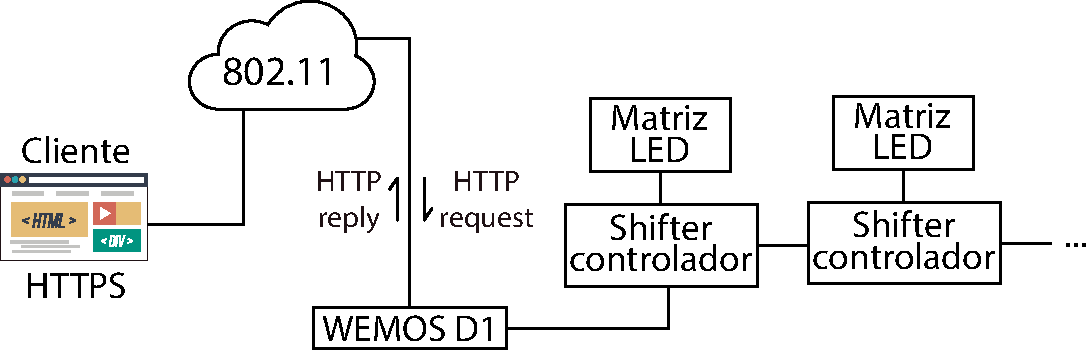
\includegraphics[width=\textwidth]{imagenes/diagrama-bloques.pdf}
		\caption{Diagrama en bloques del sistema.}
		\label{fig:Prop-Cap-response}
	\end{center}
\end{figure}


\subsection{Identificación de partes}
% a. E/S del controlador con el exterior, excepto PC 
% b. Comunicaciones con la PC 
% c. Sistema web

\begin{enumerate}[label=\alph*.]
    \item \textbf{E/S del controlador con el exterior:} debido a la baja de disponibilidad de pines que ofrece el microcontrolador, es indispensable la multiplexación con los chips de interfaz serial para el control individual de los LEDs. Para ello el microcontrolador se conecta a los Shifters MAX7219 de forma de poder controlar las matrices de LEDs de 8x8. En la figura \ref{fig:Prop-Shifter} se observa el esquema de conexión para 64 leds dispuestos en 8 filas por 8 columnas. El driver MAX7219 implementa una interfaz  SPI que consiste en un bus de comunicación a nivel de circuitos integrados en el que la transmisión de datos se realiza en serie. La comunicación con el WEMOS se realiza exclusivamente por medio de 3 pines digitales de salida (DIN, CS y CLK), además de dos pines para la alimentación (+5V) y la masa (GND).
    
    \begin{figure}[ht]
    	\centering
    	\begin{center}
    		\includegraphics[width=0.7\textwidth]{presentacion/imagenes/diagrama-shifter.png}
    		\caption{Conexión de un Shifter con una matriz de 8x8 LEDs.}
    		\label{fig:Prop-Shifter}
    	\end{center}
    \end{figure}
    
    \item \textbf{Comunicaciones:} utilizando las librerías existentes del modulo ESP8266, se configurará el microcontrolador como Access Point y como Web Server, de manera de independizar al sistema de una conexión a Internet. Entre las librearías a utilizar se encuentran ``ESP8266WebServer.h", ``WifiClient.h'' y ``ESP8266Wifi.h". Esto permitirá montar una red WIFI local y hostear un serivdor desde el microcontrolador. El programa se desarrollará bajo el framework de Arduino utilizando el lenguaje c++. Por otra parte, el manejo de las peticiones que el cliente realice, se determinarán a nivel de capa de enlace mediante el protocolo WiFi (802.11) y no será posible comunicarse con el sistema a través de un dispositivo conectado en una red externa. Dichas peticiones y respuestas se transmitirán bajo el protocolo HTTP. Las librerías previamente mencionadas permiten la implementación de este protocolo sobre el microcontrolador.
    
    \item \textbf{Sistema web:} el microcontrolador hostea una página web de manera tal que permita la comunicación entre los clientes y el WEMOS. En la figura \ref{fig:Prop-Web-text} se observa un campo de texto para que el usuario pueda ingresar una frase. En principio las letras serán estáticas, sin embargo, se plantea como objetivo secundario implementar una opción para mostrarlas a modo de marquesina.
    
    \begin{figure}[ht]
    	\centering
    	\begin{center}
    		\includegraphics[width=0.9\textwidth]{presentacion/imagenes/web-texto.png}
    		\caption{Interfaz para ingresar un texto.}
    		\label{fig:Prop-Web-text}
    	\end{center}
    \end{figure}
    
    Por otra parte, si el cliente lo desea, puede manipular los leds individualmente a través de una matriz de puntos que se encuentra en la página web. De esta forma, puede encender y apagar las luces que desee. En la figura \ref{fig:Prop-Web-matrix} se muestra la interfaz gráfica a través de la cual se implementa dicha funcionalidad.
    
    \begin{figure}[ht!]
    	\centering
    	\begin{center}
    		\includegraphics[width=0.9\textwidth]{presentacion/imagenes/web-matriz.png}
    		\caption{Interfaz para manipular LEDs individualmente.}
    		\label{fig:Prop-Web-matrix}
    	\end{center}
    \end{figure}
    
    Además los usuarios pueden elegir diferentes imágenes precargadas en la memoria del microcontrolador; dichas animaciones se pueden observar en la figura \ref{fig:Prop-Web-predefined}
    
    \begin{figure}[ht!]
    	\centering
    	\begin{center}
    		\includegraphics[width=0.9\textwidth]{presentacion/imagenes/web-predefinido.png}
    		\caption{Interfaz para elegir imágenes precargadas en memoria.}
    		\label{fig:Prop-Web-predefined}
    	\end{center}
    \end{figure}
    
    En principio las peticiones del usuario se plasman automáticamente sobre la remera de LEDs. Sin embargo se propone un objetivo secundario donde dichos pedidos se encolen en la memoria del microcontrolador. De esta forma, debería implementarse un subsistema para que el administrador, como por ejemplo, el dueño de la remera, pueda determinar qué mensajes se muestran y cuáles son descartados. Para ello se dispone de una interfaz donde el dueño pueda autenticarse y aceptar mensajes.
\end{enumerate}
    

\clearpage
\section{Código fuente Servidor Web}
El programa entero que se escribió para este proyecto se encuentra en el repositorio de github haciendo click en el \href{https://github.com/trorik23/tpii/}{link}. Adicionalmente se adjunta el material en el presente apéndice.

\subsection{main.cpp}

\lstinputlisting[caption={},
                     language=C++,
                     numbers=left,
                     escapeinside={(*@}{@*)}]
                     {codigo/src/main.cpp}
\newpage
                     
\subsection{WebServer.h}

\lstinputlisting[caption={},
                     language=C++,
                     numbers=left,
                     escapeinside={(*@}{@*)}]
                     {codigo/lib/WebServer/WebServer.h}
                     
\newpage
                     
\subsection{WebServer.cpp}

\lstinputlisting[caption={},
                     language=C++,
                     numbers=left,
                     escapeinside={(*@}{@*)}]
                     {codigo/lib/WebServer/WebServer.cpp}
                     
\newpage

\clearpage
\section{Codigo Fuente controlador matriz}
\subsection{Letter.h}

\lstinputlisting[caption={},
                     language=C++,
                     numbers=left,
                     escapeinside={(*@}{@*)}]
                     {codigo/lib/Letter/Letter.h}
                     
\newpage
                     
\subsection{Letter.cpp}

\lstinputlisting[caption={},
                     language=C++,
                     numbers=left,
                     escapeinside={(*@}{@*)}]
                     {codigo/lib/Letter/Letter.cpp}
                     
